\chapter{Программирование <<RISC>> --- цикл лабораторных работ}

Лабораторные работы по информатике посвящены арифметическим основам вычислительной техники, т.е. методам обработки символьных представлений чисел.

Указанная обработка выполняется с помощью специального RISC-процессора. RISC (reduced instruction set computing) processor --- процессор с минималистичным набором команд. Современные процессоры с избыточным набором команд, CISC\footnote{CISC --- Complex Instruction Set Computing}, в подавляющем большинстве случаев в своей основе имеют RISC-ядро. При этом сложные команды CISC-процссора реализуются подпрограммами для RISC-ядра. Таким образом, если вдруг обнаруживается ошибка в работе процессора, то её можно исправить обновлением \emph{программного обеспечения процессорного ядра}.
    
Для интерактивного проведения лабораторных работ были разработаны:
\begin{itemize}
    \item архитектура специального процессора с минималистичным набором команд\footnote{RISC --- Reduced Instruction Set Computing}, которая далее сокращенно обозначается \MyProc.
    
    \item программная модель, позволяющая создавать и отлаживать программы на языке ассемблера \MyProc.
    
    \item набор заданий, сводящийся к реализации того или иного алгоритма сложения или умножения чисел на языке ассемблера \MyProc.
\end{itemize}

Выполнение лабораторных работ позволяет студенту:
\begin{itemize}
    \item глубже понять алгоритмы работы сложных операций (умножение, деление) машинной арифметики;
    
    \item разобраться с форматами представления чисел;
    
    \item получить навыки пограммирования при ограниченных вычислительных ресурсах;
    
    \item закрепить основы логики в силу необходимости использования арифметико-логических команд для преобразования на уровне отдельных бит;
    
    \item получить навыки использования двоичной, восьмеричной и шестнадцатеричной систем счисления;
    
    \item освоить техники низкоуровневной оптимизации программ.
\end{itemize}

Классическими трудами по программированию считаются \cite{bib:knuth:artOfProgramming1,bib:knuth:artOfProgramming2,bib:knuth:artOfProgramming3}. Дональдом Кнутом, автором этих трудов, выбран подход к обучению программированию, в основе которого лежит язык ассемблера условной вычислительной машины --- MIX. Несмотря на наличие языков высокого уровня и различных высокоуровневых псеводкодов, Дональд Кнут рекомендует начинать обучение программированию с низкого уровня, а именно с языка ассемблера.

Архитектуру MIX нельзя признать простой --- её автор преследовал цели максимально компактного представления самых разных алгоритмов, которые обсуждались в его работах. В дальнейшем автором была предложена архитектура XMIX --- RISC-версия MIX. Как MIX, так и XMIX не привязаны к двоичной системе счисления.

В данном цикле лабораторных работ используется крайне минималистичная учебная архитектура \MyProc. Цели её создания: возможность работы на уровне бит и возможность реализовать рассмотренные в \cite{bib:lisikov:automateBase,bib:saveliev:automateTheory,bib:fadeeva:vmbase,bib:fadeeva:addmul} алгоритмы машинной арифметики. Также, с целью повысить качество обучения было принято решение сделать динамический выбор базисного набора RISC-команд, что позволит свести к минимуму плагиат и даст студентам возможность научиться решать задачи крайне ограниченным набором средств.
    
\section{Архитектура RISC-процессора \MyProc}
\label{ch::risc}


Преимущества RISC-архитектур в быстроте освоения програмистом, а недостатки заключаются в необходимости реализовать относительно простые операции нетривиальными подпрограммами или макроподстановками. Особенности работы с RISC исчерпывающе изложены в \cite{bib:warren:algTriks}.

\subsection{Память и адресные пространства \MyProc}

В процессоре \MyProc:
\begin{itemize}
    \item имеется 8 байтовых (8-и битных) регистров \Machine{r0},\Machine{r1},\ldots,\Machine{r7};
    \item доступна память данных из 256 8-битных ячеек с адресами от 0 до 255;
    \item оступен единственный порт ввода 8-и битного числа (см. описание команды \Opcode{in});
    \item доступен единственный порт вывода 8-и битного числа, (см. описание команды \Opcode{out});
    \item обращение к ячейке памяти данных возможно двумя способами:
    \begin{itemize}
        \item непосредственная адресация, например, <<\Machine{[0]}>> --- обращение к нулевой ячейке памяти;
        \item регистровая адресация, например, <<\Machine{[r1]}>> --- обращение к ячейке памяти с адресом, значение которого берется из регистра \Machine{r1}. Использовать для обращения к памяти можно любой из 8-и регистров.
    \end{itemize}
\end{itemize}


\subsection{Система команд \MyProc}

Архитектура {\MyProc} позволяет пользователю выбрать набор базисных команд из полного набора. Это на практике позволяет предоставить каждому студенту индивидуальный набор базисных команд. Принципы построения базисного набора инструкций изложены ниже. Полный набор команд следующий:

\begin{itemize}
    \item <<\CmdOneAddr{in}{приемник}>>. Команда ввода байта из порта ввода в \Operand{приемник}. При выполнении этой команды в программной модели {\MyProc} пользователю предлагается ввести число с экрана, которое затем заносится в \Operand{приемник}.
    
    \item <<\CmdOneAddr{out}{источник}>>. Команда записи в порт вывода. При выполнении этой команды в программной модели {\MyProc} значение байта \Operand{источник} выводится на экран.
    
    \item <<\CmdThreeAddr{ror}{источник}{количество-разрядов}{приемник}>>. Команда циклического сдвига вправо на заданное количество разрядов. \Operand{источник} циклически сдвигается на \Operand{количество-разрядов} вправо и результат сдвига записывается в \Operand{приемник}.
    
    \item <<\CmdThreeAddr{rol}{источник}{количество-разрядов}{приемник}>>. Команда циклического сдвига влево на заданное количество разрядов. \Operand{источник} циклически сдвигается на \Operand{количество-разрядов} влево и результат сдвига записывается в \Operand{приемник}.
    
    \item <<\CmdTwoAddr{not}{источник}{приемник}>>. Поразрядное логическое НЕ. Все разряды байта \Operand{источник} инвертиурются и результат записыается в \Operand{приемник}.
    
    \item <<\CmdThreeAddr{or}{источник1}{источник2}{приемник}>>. Поразрядное логическое ИЛИ. 
        \[
            \Operand{приемник} \gets \Operand{источник1} \lor \Operand{источник2}.
        \]
    
    \item <<\CmdThreeAddr{and}{источник1}{источник2}{приемник}>>. Поразрядное логическое И.
    \item <<\CmdThreeAddr{nor}{источник1}{источник2}{приемник}>>.  Поразрядное логическое ИЛИ-НЕ.
    \item <<\CmdThreeAddr{nand}{источник1}{источник2}{приемник}>>. Поразрядное логическое И-НЕ.
    \item <<\CmdThreeAddr{xor}{источник1}{источник2}{приемник}>>. Поразрядное логическое XOR.
    \item <<\CmdThreeAddr{add}{источник1}{источник2}{приемник}>>. Арифметическое сложение (с потерей переноса из старшего разряда).
    \item <<\CmdThreeAddr{sub}{источник1}{источник2}{приемник}>>. Арифметическое вычитание, соответствующее следующему сложению с потерей переноса из старшего разряда:
        \[
            \Operand{приемник} \gets \Operand{источник1} + \overline{\Operand{источник2}} + 1.
        \]
        
    \item <<\CmdTwoAddr{jz}{источник}{имя-метки}>>. Переход на метку с именем \Operand{имя-метки}, если все разряды байта \Operand{источник} равны нулю.
    \item <<\CmdTwoAddr{jo}{источник}{имя-метки}>>. Переход на метку с именем \Operand{имя-метки}, если все разряды байта \Operand{источник} равны единице.
\end{itemize}

В общем случае:
\begin{itemize}
    \item \Machine{приемник} --- это регистр или ячейка памяти, например: \Machine{r0}, \Machine{[0]}, \Machine{[r0]}, но не константа;
    \item \Machine{источник}, \Machine{количество-разрядов} --- это константа, регистр или ячейка памяти;
\end{itemize}

Все возможные базисные наборы команд определяются декартовым произведением следующих подмножеств их полного множества:
\begin{itemize}
    \item базисы команд сдвига:
        \[\{\Opcode{rol},\Opcode{ror}\};\]
    \item базисы логических команд:
        \[\{ \{\Opcode{and},\Opcode{not}\}, \{\Opcode{or},\Opcode{not}\}, \{\Opcode{and},\Opcode{xor}\}, \{\Opcode{or},\Opcode{xor}\}, \Opcode{nand},\Opcode{nor} \};\]
    \item базисы арифметических команд:
        \[\{ \Opcode{add},\Opcode{sub} \};\]
    \item базисы команд перехода:
        \[\{ \Opcode{jz},\Opcode{jo} \};\]
\end{itemize}

Для упрощения создания рабочих прототипов программ предлагается единственный избыточный набор команд $\MyProc^{(0)}$:
        \[\{ \Opcode{rol},\Opcode{ror}, \Opcode{and}, \Opcode{or}, \Opcode{not}, \Opcode{xor}, \Opcode{add},\Opcode{sub}, \Opcode{jz}, \Opcode{jo} \}, \]
от которого затем можно будет перейти к заданному набору команд.


\subsection{Язык ассемблера \MyProc}

\begin{itemize}
    \item Программа на языке ассемблера {\MyProc} оформляется в виде текстового файла, содержащего текстовые мнемоники команд \MyProc, комментарии, литералы целочисленных констант и метки.
    \item Литералы чисел могут представляться в десятичной, шестнадцатеричной (префикс <<\Machine{0x}>>), восьмеричной (префикс <<\Machine{0o}>> или <<\Machine{0}>>) и двоичной (префикс <<\Machine{0b}>>) системах счисления. Например: \Machine{10}, \Machine{0xA}, \Machine{012}, \Machine{0b1010}.
    \item Разделителем команд является перевод строки.
    \item Количество пробелов-разделителей не имеет значения.
    \item Пустые строки игнорируются.
    \item В непустой строке текстового файла может быть команда, метка или комментарий.
    \item Метка задается как <<\Machine{имя-метки:}>>.
    \item Имена меток (без двоеточия) используются в командах перехода.
    \item В программе не может двух и более меток с одинаковыми именами.
    \item Комментарий может следовать после команды или метки, признаком начала комментария всегда является символ <<\Machine{;}>>.
    \item Признаком конца комментария является перевод строки.
\end{itemize}


\subsection{Выполнение программы \MyProc}
\label{ch:risc:time}

Время, затрачиваемое на выполнение команды складывается из времени выполнения операции и времени доступа к ячейкам памяти\footnote{На практике RISC-процессор в среднем выполняет команду за один машинный такт. Это достигается за счет того, что команды просты, их размер в памяти команд одинаков, их выборка конвееризируеся и активно используется кэширование команд и данных. {\MyProc} не удовлетворяет данным требованиям. Это сделано для того, чтобы сделать очевидными критерии низкоуровневой оптимизации программ}.

Любая операция выполняется за один такт. Доступ к регистру осуществляется за один такт. Доступ к ячейке памяти осуществляется за 8 тактов. На обращение к константе (и метке в командах перехода) времени не требуется. Например, oбщее время выполнения (19 тактов) команды 
\[
    \CmdThreeAddr{add}{[r1]}{r2}{[5]}
\]
складывается как
\begin{enumerate}
    \item доступ к регистру $t(\Machine{r1})=1$;
    \item доступ к памяти $t(\Machine{[r1]})=8$;
    \item доступ к регистру $t(\Machine{r2})=1$;
    \item выполнение операции $t(\Opcode{add})=1$;
    \item доступ к памяти $t(\Machine{[5]})=8$.
\end{enumerate}

Если при выполнении команд перехода (\Opcode{jz}, \Opcode{jo}) происходит переход по метке, то на выборку новой команды процессор затрачивает 8 тактов.
 % RISC-архитектура
\section{Программирование на ассемблере \MyProc}
\label{ch::programming}

В данном разделе приводятся сведения, как можно реализовать некоторые операторы языков высокого уровня на языке ассемблера {\MyProc}. Эти сведения носят справочный характер и не означают того, что, программируя на ассемблере, следует мыслить конструкциями ЯВУ.


\subsection{Условные переходы}

Логика работы команды условного перехода проста: если оговоренное условие истинно, то выполняется переход, иначе выполняется следующая за командой перехода команда. Например, для команды \Opcode{jz} (<<если 0>>):
\begin{algorithmic}[1]
    \STATE{\CmdTwoAddr{jz}{r1}{LabelR1isZ}}
    \STATE{}\COMMENT{если $\Operand{r1}\neq 0$, то выполнятся эти команды}
    \STATE{\Operand{LabelR1isZ:}} \COMMENT{сюда выполняется переход, если $\Operand{r1}=0$}
\end{algorithmic}

Если нужен переход по инверсному условию, (в данном примере \Opcode{jnz} --- <<если не 0>>), то можно это сделать на основе имеющейся команды:
\begin{algorithmic}[1]
    \STATE{\CmdTwoAddr{jz}{r1}{LabelR1isZ}}
    \STATE{\CmdTwoAddr{jz}{0}{LabelR1isNotZ}} \COMMENT{безусловный переход!}
    \STATE{\Operand{LabelR1isZ:}} 
    \STATE{}\COMMENT{делаем что-то, при $\Operand{r1}=0$}
    \STATE{\Operand{LabelR1isNotZ:}} \COMMENT{инверсный переход! Выполняется, если $\Operand{r1}\neq 0$}
\end{algorithmic}


\subsection{Аналоги условных операторов ЯВУ}

Условный оператор на языке высокого уровня
\begin{algorithmic}[1]
    \IF {$\Operand{r1}=0$}
        \STATE{} \COMMENT{делаем что-то}
    \ELSE
        \STATE{} \COMMENT{делаем нечто}
    \ENDIF
\end{algorithmic}

на ассемблере {\MyProc} может быть реализован с помощью следующих команд:
\begin{algorithmic}[1]
    \STATE{\CmdTwoAddr{jz}{r1}{LabelFoo}}
    \STATE{}\COMMENT{делаем нечто}
    \STATE{\CmdTwoAddr{jz}{0}{LabelEndIf}}
    \STATE{\Operand{LabelFoo:}} 
    \STATE{}\COMMENT{делаем что-то}
    \STATE{\Operand{LabelEndIf:}} 
\end{algorithmic}


\subsection{Аналоги циклов ЯВУ}

\subsubsection{Цикл while}

На языке высокого уровня обычно выглядит следующим образом:
\begin{algorithmic}[1]
    \WHILE {$\Operand{r1}=0$}
        \STATE{} \COMMENT{делаем нечто}
    \ENDWHILE
\end{algorithmic}

На ассемблере он может быть реализован следующими командами:
\begin{algorithmic}[1]
    \STATE{\Operand{LabelWhileStart:}} 
    \STATE{\CmdTwoAddr{jz}{r1}{LabelWhileBody}}
    \STATE{\CmdTwoAddr{jz}{0}{LabelWhileEnd}}
    \STATE{\Operand{LabelWhileBody:}} 
    \STATE{}\COMMENT{делаем нечто}
    \STATE{\CmdTwoAddr{jz}{0}{LabelWhileStart}}
    \STATE{\Operand{LabelWhileEnd:}} 
\end{algorithmic}


\subsubsection{Цикл repeat}

\begin{algorithmic}[1]
    \REPEAT
        \STATE{} \COMMENT{делаем нечто}
    \UNTIL{$\Operand{r1}=0$}
\end{algorithmic}

на ассемблере:
\begin{algorithmic}[1]
    \STATE{\Operand{LabelRepeatStart:}} 
    \STATE{}\COMMENT{делаем нечто}
    \STATE{\CmdTwoAddr{jz}{r1}{LabelRepeatEnd}}
    \STATE{\CmdTwoAddr{jz}{0}{LabelRepeatStart}}
    \STATE{\Operand{LabelRepeatEnd:}} 
\end{algorithmic}


\subsubsection{Цикл for}

\begin{algorithmic}[1]
    \FOR{$\Operand{r1}\gets 0$ \Opcode{to} $n$}
        \STATE{} \COMMENT{делаем нечто}
    \ENDFOR
\end{algorithmic}
где $n$ --- число, на ассемблере может быть реализован следующим набором команд:

\begin{algorithmic}[1]
    \STATE{\CmdThreeAddr{add}{0}{0}{r1}}
    \STATE{\Operand{LabelForStat:}} 
    \STATE{\CmdThreeAddr{xor}{r1}{$n$}{r1}} \COMMENT{трюк: $\Operand{r1}\oplus n=0$, если $\Operand{r1}=n$}
    \STATE{\CmdTwoAddr{jz}{r1}{LabelForEnd}}
    \STATE{\CmdThreeAddr{xor}{r1}{$n$}{r1}} \COMMENT{трюк: восстанавливаем $\Operand{r1}=\Operand{r1}\oplus n\oplus n=\Operand{r1}\oplus 0$}
    \STATE{}\COMMENT{делаем нечто}
    \STATE{\CmdThreeAddr{add}{r1}{1}{r1}}
    \STATE{\CmdTwoAddr{jz}{0}{LabelForStat}} 
    \STATE{\Operand{LabelForEnd:}} 
    \STATE{\CmdThreeAddr{xor}{r1}{$n$}{r1}} \COMMENT{если $\Operand{r1}=n$ нужен далее}
\end{algorithmic}


\subsection{Вычисление формул: распространение переноса}
\label{ch:risc:p}

При сложении беззнаковых целых чисел в $n$-разрядной сетке может возникнуть ситуация ПРС, когда теряется перенос из старшего разряда. Нужно уметь определять ситуацию ПРС, так как специальных средств в {\MyProc} для этого не предусмотрено.

Пусть складываются числа $A$ и $B$ и перенос $c$:
\[
    A + B + c,
\]
где значение переноса $c$ либо 1, либо 0.

Перенос возникнет, если оба старших разряда чисел $A,B$ равны 1. Также он возникает, если старшие разряды $A,B$ различны, а старший разряд суммы $A+B+c$ получается нулевым. После вычисления выражения
\[
    (A\& B)\lor ((A \lor B) \& \lnot(A + B + c))
\]
в старшем разряде результата получается значение бита переноса.

Распределить при их нехватке регистры (или ячейки памяти) для хранения промежуточных результатов не такая уж и простая задача, даже если для всех операций находится подходящая команда:
\[
    \underbrace{
        (\underbrace{
            \overbrace{A}^\Operand{r1}
            \& 
            \overbrace{B}^\Operand{r2}
        }_\Operand{r5 (6)})
        \lor 
        \underbrace{(
            (\underbrace{
                \overbrace{A}^\Operand{r1} 
                \lor 
                \overbrace{B}^\Operand{r2}
            }_\Operand{r5 (4)})
            \& 
            \underbrace{
                \lnot
                (\underbrace{
                    \underbrace{
                        \overbrace{A}^\Operand{r1}
                        + 
                        \overbrace{B}^\Operand{r2}
                    }_\Operand{r4 (1)}
                    + 
                    \overbrace{c}^\Operand{r3}
                }_\Operand{r4 (2)})
            }_\Operand{r6 (3)}
        )}_\Operand{r6 (5)}
    }_\Operand{r5 (7)},
\]
где в подписях под фигурными скобками --- регистр, сохраняющий результат промежуточных вычислений, и (в скобках) номер команды в приведенной ниже программе, вычисляющей результат сложения и бит переноса.

\begin{algorithmic}[1]
    \REQUIRE{\Operand{r1} --- $A$, \Operand{r2} --- $B$, \Operand{r3} --- $c\in\{0,1\}$}
    \ENSURE{\Operand{r4} --- байт результата без переноса, \Operand{r5} --- перенос}
    
    \COMMENT{\Operand{r6} --- для промежуточных результатов}
    \STATE{\CmdThreeAddr{add}{r1}{r2}{r4}} \COMMENT{$\Operand{r4}\gets A+B$}
    \STATE{\CmdThreeAddr{add}{r3}{r4}{r4}} \COMMENT{$\Operand{r4}\gets A+B+c$, байт результата без переноса}
    \STATE{\CmdTwoAddr{not}{r4}{r6}} \COMMENT{$\Operand{r6}\gets \lnot(A+B+c)$}
    \STATE{\CmdThreeAddr{or}{r1}{r2}{r5}} \COMMENT{$\Operand{r5}\gets A\lor B$}
    \STATE{\CmdThreeAddr{and}{r5}{r6}{r6}} \COMMENT{$\Operand{r6}\gets (A \lor B) \& \lnot(A + B + c)$}
    \STATE{\CmdThreeAddr{and}{r1}{r2}{r5}} \COMMENT{$\Operand{r5}\gets A \& B$}
    \STATE{\CmdThreeAddr{or}{r5}{r6}{r5}} \COMMENT{$\Operand{r5}\gets (A\& B)\lor ((A \lor B) \& \lnot(A + B + c))$}
    \STATE{\CmdThreeAddr{rol}{r5}{1}{r5}} \COMMENT{признак переноса в 7-м бите r5}
    \STATE{\CmdThreeAddr{and}{r5}{1}{r5}} \COMMENT{в r5 перенос: 0 или 1}
\end{algorithmic}
  % особенности программироваиня на ассемблере
\section{Работа с программной моделью \MyProc}
\label{ch::asm}


Программная модель позволяет создавать и отлаживать программы для \MyProc. По желанию пользователя может быть установлен русский или английский язык пользовательского интерфейса.

\subsection{Главное окно приложения}

Вид главного окна приложения представлен на рисунке \ref{fig:asm:r8asmWindow}. Пользователь при желании может сменить язык интерфейса на английский, выбрав пункт меню <<Справка / Язык интерфейса / English>> и перезапустив приложение.

В строке статуса приложения (нижняя часть главного окна) пользователь может выбрать свой набор команд. Рекомендуется реализовать алгоритм в нулевом наборе, выполнить отладку и тестирование, а затем выполнить переход в свой, ограниченный набор команд.

\begin{figure}
    \centering
    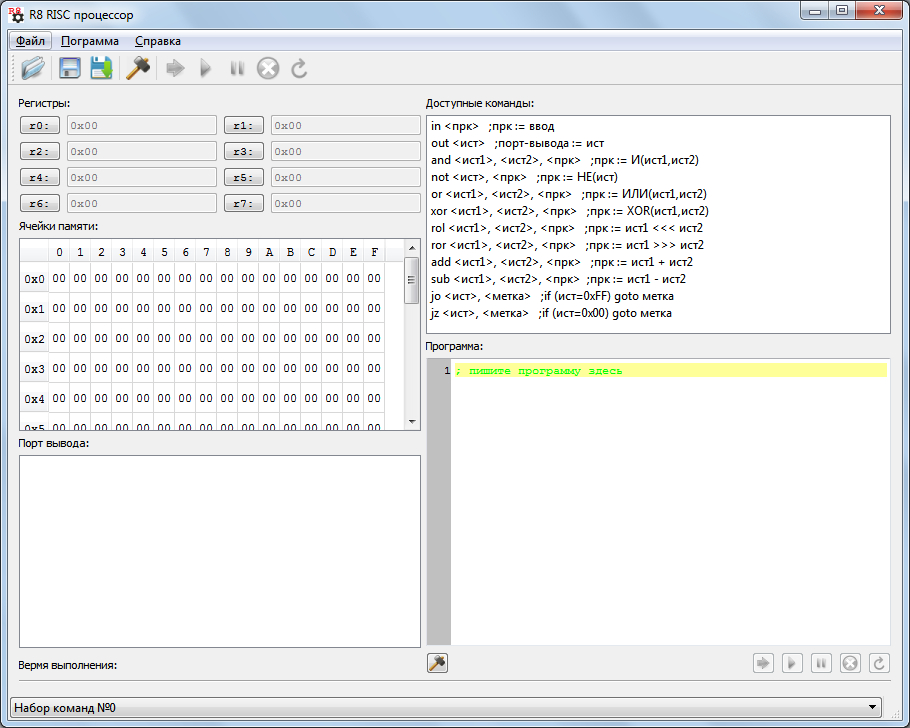
\includegraphics[width=\textwidth]{fig/r8asmWindow}
    \caption{Главное окно программной модели {\MyProc} (русский язык интерфейса)}\label{fig:asm:r8asmWindow}
\end{figure}

В главном окне программной модели отображается:
\begin{itemize}
    \item Номер текущнего набора команд RISC-процессора \MyProc.
    
    \item Состояние всех восьми регистров процессора \MyProc. Щелчок на имени регистра приводит к последовательному переключению отображения значения регистра в одну из систем счисления: двоичную, восьмеричную, шестнадцатеричную, десятичную.
    
    \item Состояние всех ячеек памяти процессора \MyProc. Значение в ячейке памяти изображается в шестнадцатеричной системе счисления.
    
    \item История вывода в порт вывода. Отображается выведенное значение в шестнадцатеричной, двоичной и десятичной системах счисления.
    
    \item Условное время выполнения программы в тактах. Правила подсчета времени выполнения приведены в разделе \ref{ch:risc:time}.
    
    \item Над областью редактора кода отображается список команд для выбранного набора с кратким описанием логики их работы.
    
    \item Область редактора позволяет в любой момент редактировать программу, отображает точки останова, а также отмечает текущую команду в режиме пошаговой отладки. Редактирование программы в процессе её отладки завершает отладку автоматически.
    
    \item Под областью редактора располагаются кнопки для выполнения основных команд отладки программы. Подробности отладки приводятся в разделе \ref{ch:asm:debug}
\end{itemize}


\subsection{Работа с редактором кода}

Редактор кода предназначен для комфортной работы с исходным текстом \MyProc-программы на языке ассемблера. Реализована подсветка синтаксиса (рисунок \ref{fig:asm:syntaxhighlight}), что облегчает редактирование программы и позволяет избежать большинства ошибок компиляции. В разном стиле подсвечиваются константы, мнемоники команд, регистры, комментарии и метки. Синтаксические ошибки подчеркиваются красной волнистой линией.

\begin{figure}
    \centering
    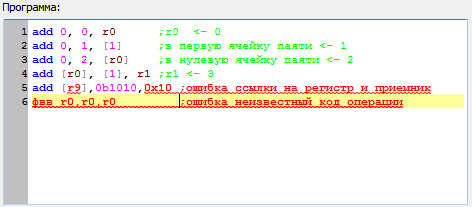
\includegraphics{fig/syntaxhighlight}
    \caption{Редактор {\MyProc} с подсветкой синтаксиса и ошибок}\label{fig:asm:syntaxhighlight}
\end{figure}

Пример отладки программы определения переноса (см. теорию в разделе \ref{ch:risc:p}) приведен на рисунке \ref{fig:asm:r8asmEditor}.

\begin{figure}
    \centering
    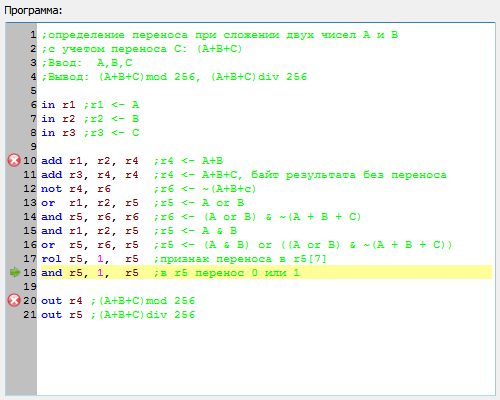
\includegraphics{fig/r8asmEditor}
    \caption{Редактор {\MyProc} в процессе отладки}\label{fig:asm:r8asmEditor}
\end{figure}

% ;определение переноса при сложении двух чисел A и B
% ;с учетом переноса С: (A+B+C)
% ;Ввод: A,B,C
% ;Вывод: (A+B+C)mod 256, (A+B+C)div 256
% ;r6 --- для промежуточных результатов
% in r1 ;r1 <- A
% in r2 ;r2 <- B
% in r3 ;r3 <- C 
%  
% add r1, r2, r4  ;r4 <- A+B
% add r3, r4, r4  ;r4 <- A+B+C, байт результата без переноса
% not r4, r6      ;r6 <- ~(A+B+c)
% or  r1, r2, r5  ;r5 <- A or B
% and r5, r6, r6  ;r6 <- (A or B) & ~(A + B + C)
% and r1, r2, r5  ;r5 <- A & B
% or  r5, r6, r5  ;r5 <- (A & B) or ((A or B) & ~(A + B))
% rol r5, 1,  r5  ;признак переноса в r5[7]
% and r5, 1,  r5  ;в r5 перенос 0 или 1
% 
% out r4 ;(A+B+C)mod 256
% out r5 ;(A+B+C)div 256

Исходный текст программы на языке ассемблера {\MyProc} можно сохранить в файл, используя соответствующие команды главного меню или кнопки на панели быстрого доступа: <<Файл / Сохранить>> или <<Файл / Сохранить как\ldots>>. Точки останова при этом не сохраняются.

Исходный текст также может быть загружен с помощью команды <<Файл / Открыть>>.


\subsection{Компиляция и отладка программы}
\label{ch:asm:debug}

Для отладки программы на языке ассемблера {\MyProc} можно выполнить следующие команды:
\begin{itemize}
    \item Перевести в машинный код (
\includegraphics[width=16pt]{fig/r8asm/image/compile}). Выполнить трансляцию мнемоник команд ассемблера {\MyProc} в машинный код {\MyProc}. Когда компиляция проходит без ошибок, становятся доступными команды отладки. Ошибки компиляции выводятся в окно порта вывода и строка, в которой обнаружена ошибка, подсвечивается.
    
    \item Выполнить команду (
\includegraphics[width=16pt]{fig/r8asm/image/step}). Пошаговый режим выполненя команд: выполняется текущая команда и выполняется останов на следующей. Текущая команда отмечается в редакторе соответствующим значком. После выполнения команды отображается новое состояние процессора.
    
    \item Выполнить программу (
\includegraphics[width=16pt]{fig/r8asm/image/run}). Выполнятеся программа целиком или выполняется переход в пошаговый режим на точке останова (
\includegraphics[width=16pt]{fig/r8asm/image/breakpoint}). 
    
    \item Останов (
\includegraphics[width=16pt]{fig/r8asm/image/stop}). Выполнятеся останов на текущей команде и переход в пошаговый режим.
    
    \item Точка останова (
\includegraphics[width=16pt]{fig/r8asm/image/breakpoint}). Выполнятеся установка точки останова в текущей строке редактора. Это не влияет на режим выполнения команд. При редактировании исходного текста, точки останова остаются в тех позициях, в которых были установлены.
    
    \item Перезапуск (
\includegraphics[width=16pt]{fig/r8asm/image/restart}). Выполнятеся сброс процессора и переход в пошаговый режим выполнения программы, начиная с первой команды.    
\end{itemize}
        % модель R8
\section{Задания на лабораторные работы}


Студент получает номер индивидуального набора команд \MyProc. С помощью команд полученного набора студенту необходимо реализовать алгоритмы основного задания. В основном задании определяется разрядность исходных данных, порядок байт и реализуемый алгоритм. 

Операнды должны быть считаны в заданном порядке из порта ввода. Результат  должен быть выведен в порт вывода, также в заданном порядке.

\subsection{Задания на первую лабораторную работу}

В порядке ознакомления с программной моделью {\MyProc} студенту предлагается реализовать следующие алгоритмы.

\begin{itemize}
    \item Сброс $n$-го бита в 8-разрядном числе.
    \item Перевод 8-разрядного числа из прямого кода в дополнительный.
    \item Сложение двух 16-разрядных чисел в дополнительном коде. Порядок байт --- little-endian.
    \item Подсчет единичных бит в 16-разрядном числе.
    \item Сравнение 16-разрядных чисел $A$ и $B$, представленных в дополнительном коде. Порядок байт --- big-endian. Вывести:
    \[
        \begin{cases}
            -1, &\text{если $A<B$};\\
             0, &\text{если $A=B$};\\
            +1, &\text{если $A>B$}.
        \end{cases}
    \]
    \item Сдвиг 16-разрядного дополнительного кода числа на один разряд вправо. Порядок байт --- little-endian.
    \item Сдвиг 16-разрядного обратного кода числа на один разряд влево. Порядок байт --- big-endian.
\end{itemize}


\subsection{Задания на вторую лабораторную работу}

Вторая лабораторная работа предназначена для закрепления теоретического материала по арифметическим основам ЭВМ. 
На выбор предлагаются следующие группы заданий:
\begin{itemize}
    \item Умножение чисел в формате с фиксированной точкой.
    \item Сложение чисел в формате с плавающей точкой.
    \item Умножение чисел в формате с плавающей точкой.
\end{itemize}

Студенту необходимо получить номер варианта в рамках выбранной группы заданий и реализовать соответствующий алгоритм.

Варианты заданий для умножения чисел в формате с фиксированной точкой:
\begin{enumerate}
    \item Алгоритм умножения 8-разрядных беззнаковых чисел I-м способом.
    \item Алгоритм умножения 8-разрядных беззнаковых чисел II-м способом.
    \item Алгоритм умножения 8-разрядных беззнаковых чисел III-м способом.
    \item Алгоритм умножения 8-разрядных беззнаковых чисел IV-м способом.
    \item Алгоритм умножения 8-разрядных беззнаковых чисел с ускорением второго порядка I-м способом.
    \item Алгоритм умножения 8-разрядных беззнаковых чисел с ускорением второго порядка II-м способом.
    \item Алгоритм умножения 8-разрядных беззнаковых чисел с ускорением второго порядка III-м способом.
    \item Алгоритм умножения 8-разрядных беззнаковых чисел с ускорением второго порядка IV-м способом.
    \item Алгоритм умножения 8-разрядных чисел в дополнительном коде с автоматической коррекцией I-м способом.
    \item Алгоритм умножения 8-разрядных чисел в дополнительном коде с автоматической коррекцией II-м способом.
    \item Алгоритм умножения 8-разрядных чисел в дополнительном коде с автоматической коррекцией III-м способом.
    \item Алгоритм умножения 8-разрядных чисел в дополнительном коде с автоматической коррекцией IV-м способом.
    \item Алгоритм умножения 8-разрядных чисел в дополнительном коде с простой коррекцией I-м способом.
    \item Алгоритм умножения 8-разрядных чисел в дополнительном коде с простой коррекцией II-м способом.
    \item Алгоритм умножения 8-разрядных чисел в дополнительном коде с простой коррекцией III-м способом.
    \item Алгоритм умножения 8-разрядных чисел в дополнительном коде с простой коррекцией IV-м способом.
    \item Алгоритм умножения 16-разрядных беззнаковых чисел I-м способом.
    \item Алгоритм умножения 16-разрядных беззнаковых чисел II-м способом.
    \item Алгоритм умножения 16-разрядных беззнаковых чисел III-м способом.
    \item Алгоритм умножения 16-разрядных беззнаковых чисел IV-м способом.
    \item Алгоритм умножения 16-разрядных беззнаковых чисел с ускорением второго порядка I-м способом.
    \item Алгоритм умножения 16-разрядных беззнаковых чисел с ускорением второго порядка II-м способом.
    \item Алгоритм умножения 16-разрядных беззнаковых чисел с ускорением второго порядка III-м способом.
    \item Алгоритм умножения 16-разрядных беззнаковых чисел с ускорением второго порядка IV-м способом.
    \item Алгоритм умножения 16-разрядных чисел в дополнительном коде с автоматической коррекцией I-м способом.
    \item Алгоритм умножения 16-разрядных чисел в дополнительном коде с автоматической коррекцией II-м способом.
    \item Алгоритм умножения 16-разрядных чисел в дополнительном коде с автоматической коррекцией III-м способом.
    \item Алгоритм умножения 16-разрядных чисел в дополнительном коде с автоматической коррекцией IV-м способом.
    \item Алгоритм умножения 16-разрядных чисел в дополнительном коде с простой коррекцией I-м способом.
    \item Алгоритм умножения 16-разрядных чисел в дополнительном коде с простой коррекцией II-м способом.
    \item Алгоритм умножения 16-разрядных чисел в дополнительном коде с простой коррекцией III-м способом.
    \item Алгоритм умножения 16-разрядных чисел в дополнительном коде с простой коррекцией IV-м способом.
\end{enumerate}

Варианты заданий для сложения чисел в формате с плавающей точкой:
\begin{enumerate}
    \item Алгоритм сложения чисел в 16-разрядном формате с плавающей точкой. Форматом используется характеристика. Для представления мантиссы используется прямой код. Остальные особенности формата и соглашение о порядке следования байт (little-endian, big-endian) разрабатываются студентом самостоятельно.
    \item Алгоритм сложения чисел в 16-разрядном формате с плавающей точкой. Форматом используется характеристика. Для представления мантиссы используется дополнительный код. Остальные особенности формата и соглашение о порядке следования байт (little-endian, big-endian) разрабатываются студентом самостоятельно.
    \item Алгоритм сложения чисел в 16-разрядном формате с плавающей точкой. Форматом используется характеристика. Для представления мантиссы используется обратный код. Остальные особенности формата и соглашение о порядке следования байт (little-endian, big-endian) разрабатываются студентом самостоятельно.
    \item Алгоритм сложения чисел в 16-разрядном формате с плавающей точкой. Форматом используется порядок. Для представления мантиссы используется прямой код. Остальные особенности формата и соглашение о порядке следования байт (little-endian, big-endian) разрабатываются студентом самостоятельно.
    \item Алгоритм сложения чисел в 16-разрядном формате с плавающей точкой. Форматом используется порядок. Для представления мантиссы используется дополнительный код. Остальные особенности формата и соглашение о порядке следования байт (little-endian, big-endian) разрабатываются студентом самостоятельно.
    \item Алгоритм сложения чисел в 16-разрядном формате с плавающей точкой. Форматом используется порядок. Для представления мантиссы используется обратный код. Остальные особенности формата и соглашение о порядке следования байт (little-endian, big-endian) разрабатываются студентом самостоятельно.
    \item Алгоритм сложения чисел в 24-разрядном формате с плавающей точкой. Форматом используется характеристика. Для представления мантиссы используется прямой код. Остальные особенности формата и соглашение о порядке следования байт (little-endian, big-endian) разрабатываются студентом самостоятельно.
    \item Алгоритм сложения чисел в 24-разрядном формате с плавающей точкой. Форматом используется характеристика. Для представления мантиссы используется дополнительный код. Остальные особенности формата и соглашение о порядке следования байт (little-endian, big-endian) разрабатываются студентом самостоятельно.
    \item Алгоритм сложения чисел в 24-разрядном формате с плавающей точкой. Форматом используется характеристика. Для представления мантиссы используется обратный код. Остальные особенности формата и соглашение о порядке следования байт (little-endian, big-endian) разрабатываются студентом самостоятельно.
    \item Алгоритм сложения чисел в 24-разрядном формате с плавающей точкой. Форматом используется порядок. Для представления мантиссы используется прямой код. Остальные особенности формата и соглашение о порядке следования байт (little-endian, big-endian) разрабатываются студентом самостоятельно.
    \item Алгоритм сложения чисел в 24-разрядном формате с плавающей точкой. Форматом используется порядок. Для представления мантиссы используется дополнительный код. Остальные особенности формата и соглашение о порядке следования байт (little-endian, big-endian) разрабатываются студентом самостоятельно.
    \item Алгоритм сложения чисел в 24-разрядном формате с плавающей точкой. Форматом используется порядок. Для представления мантиссы используется обратный код. Остальные особенности формата и соглашение о порядке следования байт (little-endian, big-endian) разрабатываются студентом самостоятельно.
\end{enumerate}

Варианты заданий для умножения чисел в формате с плавающей точкой:
\begin{enumerate}
    \item Алгоритм умножения чисел в 16-разрядном формате с плавающей точкой. Форматом используется характеристика. Для представления мантиссы используется прямой код. Перемножение мантисс выполняется I способом умножения. Остальные особенности формата и соглашение о порядке следования байт (little-endian, big-endian) разрабатываются студентом самостоятельно.
    \item Алгоритм умножения чисел в 16-разрядном формате с плавающей точкой. Форматом используется характеристика. Для представления мантиссы используется прямой код. Перемножение мантисс выполняется II способом умножения. Остальные особенности формата и соглашение о порядке следования байт (little-endian, big-endian) разрабатываются студентом самостоятельно.
    \item Алгоритм умножения чисел в 16-разрядном формате с плавающей точкой. Форматом используется характеристика. Для представления мантиссы используется прямой код. Перемножение мантисс выполняется III способом умножения. Остальные особенности формата и соглашение о порядке следования байт (little-endian, big-endian) разрабатываются студентом самостоятельно.
    \item Алгоритм умножения чисел в 16-разрядном формате с плавающей точкой. Форматом используется характеристика. Для представления мантиссы используется прямой код. Перемножение мантисс выполняется IV способом умножения. Остальные особенности формата и соглашение о порядке следования байт (little-endian, big-endian) разрабатываются студентом самостоятельно.
    \item Алгоритм умножения чисел в 16-разрядном формате с плавающей точкой. Форматом используется характеристика. Для представления мантиссы используется дополнительный код. Перемножение мантисс выполняется I способом умножения. Остальные особенности формата и соглашение о порядке следования байт (little-endian, big-endian) разрабатываются студентом самостоятельно.
    \item Алгоритм умножения чисел в 16-разрядном формате с плавающей точкой. Форматом используется характеристика. Для представления мантиссы используется дополнительный код. Перемножение мантисс выполняется II способом умножения. Остальные особенности формата и соглашение о порядке следования байт (little-endian, big-endian) разрабатываются студентом самостоятельно.
    \item Алгоритм умножения чисел в 16-разрядном формате с плавающей точкой. Форматом используется характеристика. Для представления мантиссы используется дополнительный код. Перемножение мантисс выполняется III способом умножения. Остальные особенности формата и соглашение о порядке следования байт (little-endian, big-endian) разрабатываются студентом самостоятельно.
    \item Алгоритм умножения чисел в 16-разрядном формате с плавающей точкой. Форматом используется характеристика. Для представления мантиссы используется дополнительный код. Перемножение мантисс выполняется IV способом умножения. Остальные особенности формата и соглашение о порядке следования байт (little-endian, big-endian) разрабатываются студентом самостоятельно.
    \item Алгоритм умножения чисел в 16-разрядном формате с плавающей точкой. Форматом используется порядок. Для представления мантиссы используется прямой код. Перемножение мантисс выполняется I способом умножения. Остальные особенности формата и соглашение о порядке следования байт (little-endian, big-endian) разрабатываются студентом самостоятельно.
    \item Алгоритм умножения чисел в 16-разрядном формате с плавающей точкой. Форматом используется порядок. Для представления мантиссы используется прямой код. Перемножение мантисс выполняется II способом умножения. Остальные особенности формата и соглашение о порядке следования байт (little-endian, big-endian) разрабатываются студентом самостоятельно.
    \item Алгоритм умножения чисел в 16-разрядном формате с плавающей точкой. Форматом используется порядок. Для представления мантиссы используется прямой код. Перемножение мантисс выполняется III способом умножения. Остальные особенности формата и соглашение о порядке следования байт (little-endian, big-endian) разрабатываются студентом самостоятельно.
    \item Алгоритм умножения чисел в 16-разрядном формате с плавающей точкой. Форматом используется порядок. Для представления мантиссы используется прямой код. Перемножение мантисс выполняется IV способом умножения. Остальные особенности формата и соглашение о порядке следования байт (little-endian, big-endian) разрабатываются студентом самостоятельно.
    \item Алгоритм умножения чисел в 16-разрядном формате с плавающей точкой. Форматом используется порядок. Для представления мантиссы используется дополнительный код. Перемножение мантисс выполняется I способом умножения. Остальные особенности формата и соглашение о порядке следования байт (little-endian, big-endian) разрабатываются студентом самостоятельно.
    \item Алгоритм умножения чисел в 16-разрядном формате с плавающей точкой. Форматом используется порядок. Для представления мантиссы используется дополнительный код. Перемножение мантисс выполняется II способом умножения. Остальные особенности формата и соглашение о порядке следования байт (little-endian, big-endian) разрабатываются студентом самостоятельно.
    \item Алгоритм умножения чисел в 16-разрядном формате с плавающей точкой. Форматом используется порядок. Для представления мантиссы используется дополнительный код. Перемножение мантисс выполняется III способом умножения. Остальные особенности формата и соглашение о порядке следования байт (little-endian, big-endian) разрабатываются студентом самостоятельно.
    \item Алгоритм умножения чисел в 16-разрядном формате с плавающей точкой. Форматом используется порядок. Для представления мантиссы используется дополнительный код. Перемножение мантисс выполняется IV способом умножения. Остальные особенности формата и соглашение о порядке следования байт (little-endian, big-endian) разрабатываются студентом самостоятельно.
\end{enumerate}
        % задания на лабораторную работу
